%
%===============>>  ГРУППА 11-4 МОДУЛЬ 8  <<=============
%
\setmodule{8}

%BEGIN_FOLD % ====>>_____ Занятие 1 _____<<====
\begin{class}[number=1]
	\begin{listofex}
		\item Постройте график уравнения:
		\begin{tasks}(2)
			\task \( xy-2=2x-y \)
			\task \( y\sqrt{x}-1=y-\sqrt{x} \)
			\task \( (x^2+4)(y^2+1)=8xy \)
			\task \( (y-2)^2=(x+1)^2 \)
			\task \( |y|=2-x \)
			\task \( |y|=9-x^2 \)
			\task \( x|y|=-2 \)
			\task \( |y|(x+1)=1 \)
			\task \( |y|=2|x|-x^2 \)
			\task \( |y|=x^2-4|x|+3 \)
			\task \( |y|=|x^2-4x+3| \)
			\task \( x^2-6x+9=y^4 \)
		\end{tasks}
		\item Изобразите на координатной плоскости множество точек, координаты которых \( (x; y) \) удовлетворяют неравенству:
		\begin{tasks}(2)
			\task \( (x-1)(y+2)\ge0 \)
			\task \( (x-1)(|y|+2)\le0 \)
			\task \( x^2\ge y^2 \)
			\task \( y>3|x|-2 \)
			\task \( y\le|2-\sqrt{x+1}| \)
			\task \( |x|+|y|\le3 \)
		\end{tasks}
%		\item Найдите все значения параметра \( a \), при каждом из которых система уравнений
%		\[ \left\{
%		\begin{array}{l}
%			x^2-2x+|y|-15=0,\\
%			x^2+(y-a)(y+a)=2\left( x-\dfrac{1}{2} \right)
%		\end{array}
%		\right. \]
%		имеет ровно 6 решений.
		\item Найдите все значения параметра \( a \), при каждом из которых система уравнений
		\[ \left\{
		\begin{array}{l}
			(y^2-xy+x-3y+2)\sqrt{x+3}=0,\\
			a-x-y=0
		\end{array}
		\right. \]
		имеет ровно два различных решения.
		\item Найдите все значения параметра \( a \), при каждом из которых система уравнений
		\[ \left\{
		\begin{array}{l}
			4|y-3|=12-3|x|,\\
			y^2-a^2=3(2y-3)-x^2
		\end{array}
		\right. \]
		имеет ровно четыре решения.
		\item Для каждого значения параметра \( a \) решить уравнение:
		\[ |x+a|+|x-a|=2 \]
	\end{listofex}
\end{class}
%END_FOLD

%BEGIN_FOLD % ====>>_____ Занятие 2 _____<<====
\begin{class}[number=2]
	\begin{listofex}
		\item Найдите все значения \(a\), при каждом из которых система \[ \begin{cases} yx^2+y^2=2y+63-7x^2, \\ x \ge -3, \\ x+y=a  \end{cases} \] имеет ровно два различных решения.
		\item Найдите все значения \(a\), при каждом из которых система \[ \begin{cases} x^2-2x+|y|-15=0 \\ x^2+(y-a)(y+a)=2 (x-0,5)  \end{cases} \] имеет ровно шесть решений.
		\item Найдите все значения \(a\), при каждом из которых система уравнений \[ \begin{cases} |x-4|+3|y|=2 \\ 9y^2+x^2-8x+4(a+3)=0 \end{cases} \] имеет ровно четыре решения.
	\end{listofex}
\end{class}
%END_FOLD

%BEGIN_FOLD % ====>>_ Домашняя работа 1 _<<====
\begin{homework}[number=1]
	\begin{listofex}
		\item Имеются два сосуда. Первый содержит \( 30 \) кг, а второй --- \( 20 \) кг раствора кислоты различной концентрации. Если эти растворы смешать, то получится раствор, содержащий \( 68\% \) кислоты. Если же смешать равные массы этих растворов, то получится раствор, содержащий \( 70\% \) кислоты. Сколько килограммов кислоты содержится в первом сосуде?
		\item Найдите наибольшее значение функции \( y=x+\dfrac{9}{x} \) на отрезке \( [-4; -1] \)
		\item 
		\begin{tasks}(1)
			\task Решите уравнение: \( \log_4\left( 2^{2x}-\sqrt{3}\cos x-\sin2x \right)=x \).
			\task Найжите все корни этого уравнения, принадлежащие отрезку \( \left[ 2\pi; \dfrac{7\pi}{2} \right]  \).
		\end{tasks}
		\item Решите неравенство \( \dfrac{0,2^{|x^2-4x+2|}-0,04}{3-x}\le0 \).
		\item Найдите все значения параметра \( a \), при каждом из которых система уравнений
		\[ \begin{cases}
			3|x-2|+|y|-3=0,\\
			ax-y+2a+2=0
		\end{cases} \]
		имеет ровно \( 2 \) решения.
		\item Найдите все значения параметра \( a \), при каждом из которых система уравнений
		\[ \begin{cases}
			\dfrac{xy^2-2xy-4y+8}{\sqrt{x+4}}=0,\\
			y=ax
		\end{cases} \]
		имеет ровно \( 2 \) различных решения.
		\item Найдите все значения параметра \( a \), при каждом из которых система уравнений
		\[ \begin{cases}
			x^2+12x+|y|+27=0,\\
			x^2+(y-a)(y+a)=-12(x+3)
		\end{cases} \]
		имеет ровно \( 4 \) решения.
	\end{listofex}
\end{homework}
%END_FOLD

%BEGIN_FOLD % ====>>_____ Занятие 3 _____<<====
\begin{class}[number=3]
	\begin{listofex}
		\item
		\begin{minipage}[t]{\bodywidth}
			Биссектриса тупого угла параллелограмма делит противоположную сторону в отношении \( 4 : 3 \), считая от вершины острого угла. Найдите большую сторону параллелограмма, если его периметр равен \( 88 \).
			\foranswer
		\end{minipage}
		\gapwidth
		\begin{minipage}[t]{\picwidth}
			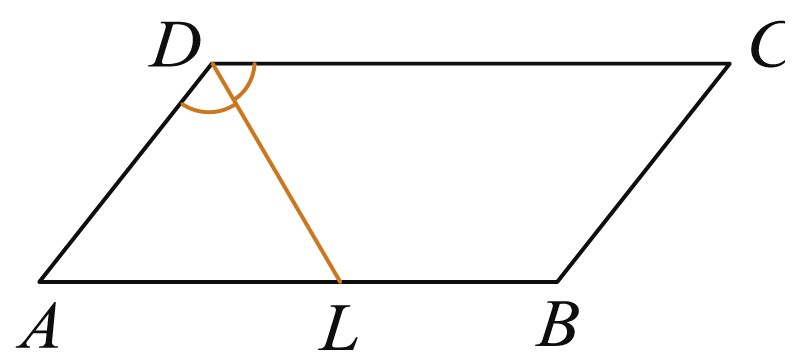
\includegraphics[align=t, width=\linewidth]{\picpath/prob_3_1}
		\end{minipage}
		\item
		\begin{minipage}[t]{\bodywidth}
			Площадь боковой поверхности конуса в два раза больше площади основания. Найдите угол между образующей конуса и плоскостью основания. Ответ дайте в градусах.
			\foranswer
		\end{minipage}
		\gapwidth
		\begin{minipage}[t]{\picwidth}
			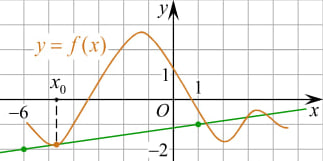
\includegraphics[align=t, width=\linewidth]{\picpath/prob_3_2}
		\end{minipage}
		\item У Дины в копилке лежит \( 7 \) рублёвых, \( 5 \) двухрублёвых, \( 6 \) пятирублёвых и \( 2 \) десятирублёвых
		монеты. Дина наугад достаёт из копилки одну монету. Найдите вероятность того, что оставшаяся в
		копилке сумма составит менее \( 60 \) рублей.
		\foranswer
		\item Чтобы пройти в следующий круг соревнований, футбольной команде нужно набрать хотя бы \( 4 \)
		очка в двух играх. Если команда выигрывает, она получает \( 3 \) очка, в случае ничьей --- \( 1 \) очко, если
		проигрывает --- \( 0 \) очков.
		Найдите вероятность того, что команде удастся выйти в следующий круг
		соревнований.
		Считайте, что в каждой игре вероятности выигрыша и проигрыша одинаковы и равны \( 0,4 \).
		\foranswer
		\item Решите уравнение \( \sin \dfrac{\pi x}{3}=0,5 \). В ответе напишите наименьший положительный корень.
		\foranswer
		\item Найдите значение выражения \( 0,8^{1/7}\cdot5^{2/7}\cdot20^{6/7} \).
		\item
		\begin{minipage}[t]{\bodywidth}
			На рисунке изображены график функции \( y=f(x) \) и касательная к этому графику, проведенная в точке \( x_0 \). Уравнение касательной показано на рисунке. Найдите значение функции \( g(x)=(f`(x)-0,5)\cdot6 \) в точке \( x_0 \).
			\foranswer
		\end{minipage}
		\gapwidth
		\begin{minipage}[t]{\picwidth}
			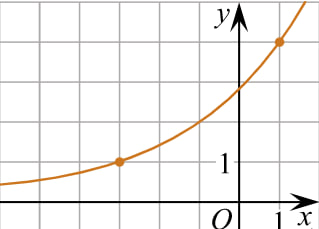
\includegraphics[align=t, width=\linewidth]{\picpath/prob_3_3}
		\end{minipage}
	\item Автомобиль, масса которого равна \( m=2160 \) кг, начинает двигаться с ускорением, которое в
	течение \( t \) секунд остаeтся неизменным, и проходит за это время путь \( S=500 \) метров. Значение силы
	(в ньютонах), приложенной в это время к автомобилю, равно \( F=\dfrac{2mS}{t^2} \). Определите наибольшее
	время после начала движения автомобиля, за которое он пройдeт указанный путь, если известно, что
	сила \( F \), приложенная к автомобилю, не меньше \( 2400 \) H. Ответ выразите в секундах.
	\foranswer
	\item Петя и Ваня выполняют одинаковый тест. Петя отвечает за час на 8 вопросов теста, а Ваня —
	на 9. Они одновременно начали отвечать на вопросы теста, и Петя закончил свой тест позже Вани на
	20 минут. Сколько вопросов содержит тест?
	\foranswer
	\item
	\begin{minipage}[t]{\bodywidth}
		На рисунке изображён график функции вида \( f(x)=\dfrac{a}{x+b}+c \), где числа \( a \), \( b \), \( c \) -- целые числа. Найдите \( f\left( \dfrac{4}{3} \right) \).
		\foranswer
	\end{minipage}
	\gapwidth
	\begin{minipage}[t]{\picwidth}
		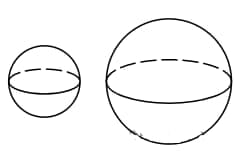
\includegraphics[align=t, width=\linewidth]{\picpath/prob_3_4}
	\end{minipage}
	\item Найдите точку минимума функции \( y=2x-\ln(x+3)+7 \).
	\foranswer
	\item Найдите все значения \( a \), для каждого из которых уравнение \[ \log_{1-x}(a-x+2)=2 \] имеет хотя бы один корень, принадлежащий промежутку \( [-1;1) \).
	\end{listofex}
	\newpage
	\begin{listofex}
	\item Найдите все значения параметра \( a \), при каждом из которых уравнение
	\[ x^2-x-a=0 \]
	имеет хотя бы одно решение, удовлетворяющее неравенству \( x>\dfrac{1}{2} \).
	\item При каких значениях параметра \( a \) все решения уравнения
	\[ 3|x+2a|-3a+x-15=0 \]
	удовлетворяют неравенству \( 4\le x \le 6 \)?
	\item Найдите все значения параметра a, при каждом из которых на интервале \( (1;2) \) существует хотя бы одно число \( x \), неудовлетворяющее неравенству
	\[ a + \sqrt{a^2-2ax+x^2}\le3x-x^2. \]
	\item Найдите все значения \( а \), при каждом из которых система неравенств
	\[ \left\{
	\begin{array}{l}
		ax\ge2,\\
		\sqrt{x-1}>a,\\
		3x\le2a+11
	\end{array}
	\right. \]
	имеет хотя бы одно решение на отрезке \( [3;4] \).
	\item Найдите все положительные значения \( a \), при каждом из которых множеством решений неравенства
	\[ \dfrac{x-2}{ax^2-(a^2+1)x+a}\ge0 \]
	является некоторый луч.
	\end{listofex}
\end{class}
%END_FOLD

%BEGIN_FOLD % ====>>_____ Занятие 4 _____<<====
\begin{class}[number=4]
	\begin{listofex}
		\item Найдите все значения \( a \), при каждом из которых система неравенств
		\[ \left\{
		\begin{array}{l}
			(a+7x+4)(a-2x+4)\le0,\\
			a+3x\ge x^2
		\end{array}
		\right. \]
		имеет хотя бы одно решение.
		\item Найдите все значения \( a \), при каждом из которых неравенство
		\[ \left|\dfrac{x^2+x-2a}{x+a}-1\right|\le2 \]
		не имеет решений на интервале \( (1;2) \).
		\item Решите неравенство: \( \dfrac{9^x-3^x-90}{3^x-82}\le1 \).
		\item Решите неравенство: \( \dfrac{3^{|x^2-2x-1|}}{x}\ge0 \).
	\end{listofex}
\end{class}
%END_FOLD

%BEGIN_FOLD % ====>>_ Домашняя работа 2 _<<====
\begin{homework}[number=2]
	\begin{listofex}
		\item Найдите наибольшее значение функции \( y=\ln(x+5)^5-5x \) на отрезке \( [-4,5;0] \).
		\item
		а) Решите уравнение \( |2\tg x - 5| - |2\tg x - 1|=2 \)\\
		б) Укажите корни этого уравнения, принадлежащие отрезку \( \left[ -\dfrac{\pi}{2};\dfrac{\pi}{2} \right] \).
		\item Решите неравенство \( \sqrt{3\cdot4^x-5\cdot2^{x+1}+3}\ge2^x-3 \).
		\item Найдите все значения параметра \( a \), при каждом из которых система неравенств
		\[ \left\{
		\begin{array}{l}
			a+3x\le12,\\
			a+4x\ge x^2,\\
			a\le x
		\end{array}
		\right. \]
		имеет хотя бы одно решение.
		\item Найдите все значения параметра a, при каждом из которых хотя бы одно решение неравенства
		\( x^2+a+|x-a-1|+1\le3x \) принадлежит отрезку \( [0;1] \).
		\item Найдите все решения параметра \( a \), при которых уравнение
		\[ x^2-4x-2|x-a|+2+a=0 \]
		имеет ровно два решения.
		\item Найдите все значения параметра \( a \), при каждом из которых неравенство
		\[ \dfrac{x-3a-1}{x+2a-2}\le0 \]
		выполняется для всех \( x \) из промежутка \( 2\le x\le3 \).
	\end{listofex}
\end{homework}
%END_FOLD

%BEGIN_FOLD % ====>>_____ Занятие 5 _____<<====
\begin{class}[number=5]
	\begin{listofex}
		\item Найдите все значения параметра \( a \), при каждом из которых уравнение
		\[ |x^2+a^2-5x-4a|=x+a \]
		имеет \( 4 \) решения.
		\rightlabel{Реальный ЕГЭ 02.06.2022}
		\item Найдите все значения параметра \( a \), при каждом из которых уравнение
		\[ |x^2-a^2|=|x+a|\cdot\sqrt{x^2-ax+4a} \]
		имеет два различных корня.
		\rightlabel{Реальный ЕГЭ 07.06.2021}
		\item Найдите все значения параметра \( a \), при каждом из которых уравнение
		\[ \dfrac{|4x|-x-3-a}{x^2-x-a}=0 \]
		имеет ровно два различных корня.
		\rightlabel{Реальный ЕГЭ 2019 г.}
		\item Найдите все значения параметра \( a \), при каждом из которых система уравнений
		\[ \left\{
		\begin{array}{l}
			x^2+y^2-4(a+1)x-2ay+5a^2+8a+3=0,\\
			y^2=x^2
		\end{array}
		\right. \]
		имеет ровно четыре различных решения.
		\rightlabel{Реальный ЕГЭ 2018 г.}
		\item Найдите все значения параметра \( a \), при каждом из которых уравнение
		\[\ln(3a-x)\ln(2x+2a-5)=\ln(3a-x)\ln(x-a) \]
		имеет ровно один корень на отрезке \( [0;2] \).
		\rightlabel{Реальный ЕГЭ 2017 г.}
		\item Найдите все значения параметра \( a \), при каждом из которых система уравнений
		\[ \left\{
		\begin{array}{l}
			(x-3)(y+3x-9)=|x-3|^3,\\
			y=x+a
		\end{array}
		\right. \]
		имеет ровно четыре различных решения.
		\rightlabel{Реальный ЕГЭ 2016 г.}
		\item Найдите все значения параметра \( a \), при каждом из которых система уравнений
		\[ \left\{
		\begin{array}{l}
			y^2+x-2=|x^2+x-2|,\\
			x-y=a
		\end{array}
		\right. \]
		имеет более двух решений.
		\rightlabel{Реальный ЕГЭ 2015 г.}
		\item Найдите все значения параметра \( a \), при каждом из которых система уравнений
		\[ \left\{
		\begin{array}{l}
			\sqrt{16-y^2}=\sqrt{16-a^2x^2},\\
			x^2+y^2=8x+4y
		\end{array}
		\right. \]
		имеет ровно два различных корня.
		\rightlabel{Реальный ЕГЭ 10.07.2020}
	\end{listofex}
\end{class}
%END_FOLD

%BEGIN_FOLD % ====>>_____ Занятие 6 _____<<====
\begin{class}[number=6]
	\begin{listofex}
		\item
		а) Решите уравнения \( \cos2x+\sqrt{2}\cos\left( \dfrac{\pi}{2}-x \right)-1=0 \);\\
		б) Укажите корни этого уравнения, принадлежащие отрезку \( \left[ \dfrac{5\pi}{2};4\pi \right] \).
		\item Решить неравенство:
		\[ x^2\cdot\log_{625}(3-x)\le\log_5(x^2-6x+9) \]
		\item Найдите все значения параметра \( a \), при каждом из которых система уравнений
		\[ \left\{
		\begin{array}{l}
			\log_3(a-x^2)=\log_3(a-y^2),\\
			x^2+y^2=4x+6y
		\end{array}
		\right. \]
		имеет ровно два различных решения.
		\item Найдите все значения параметра \( a \), при каждом из которых система уравнений
		\[ \left\{
		\begin{array}{l}
			(x-3)(y+3x-9)=|x-3|^3,\\
			y=x+a
		\end{array}
		\right. \]
		имеет ровно четыре различных решения.
		\rightlabel{Реальный ЕГЭ 2016 г.}
		\item 15-го января планируется взять кредит в банке на 19 месяцев. Условия его возврата таковы:\\
		--- 1-го числа каждого месяца долг возрастёт на \( r\% \) по сравнению с концом предыдущего месяца;\\
		--- со 2-го по 14-е число каждого месяца необходимо выплатить часть долга;\\
		--- 15-го числа каждого месяца долг должен быть на одну и ту же сумму меньше долга на 15-е число предыдущего месяца.\\
		Известно, что общая сумма выплат после полного погашения кредита на 30\% больше суммы, взятой в кредит. Найдите \( r \).
		\item 31 декабря 2013 года Сергей взял в банке \( 9\;930\;000 \) рублей в кредит под \( 10\% \) годовых. Схема выплаты кредита следующая: 31 декабря каждого следующего года банк начисляет проценты на оставшуюся сумму долга (то есть увеличивает долг на \( 10\% \)), затем Сергей переводит в банк определённую сумму ежегодного платежа. Какой должна быть сумма ежегодного платежа, чтобы Сергей выплатил долг тремя равными ежегодными платежами?
	\end{listofex}
\end{class}
%END_FOLD

%BEGIN_FOLD % ====>>_ Домашняя работа 3 _<<====
\begin{homework}[number=3]
	\begin{listofex}
		\item
		а) Решите уравнения
		\( 2\sin^2(x+\pi)-\cos\left( \dfrac{\pi}{2}-x \right)=0 \);\\
		б) Укажите корни этого уравнения, принадлежащие отрезку
		\( \left[ -\dfrac{5\pi}{2};-\pi \right] \).
		\item Решить неравенство:
		\[ x^2\cdot\log_{243}(x+6)\le\log_3(x^2+12x+36) \]
		\item Решить неравенство:
		\[ \dfrac{9^x-3^{x+1}-19}{3^x-6}+\dfrac{9^{x+1}-3^{x+4}+2}{3^x-9}\le10\cdot3^x+3 \]
		\item Найдите все значения параметра \( a \), при каждом из которых система уравнений
		\[ \left\{
		\begin{array}{l}
			\sqrt{36-y^2}=\sqrt{36-a^2x^2},\\
			x^2+y^2=6x+8y
		\end{array}
		\right. \]
		имеет ровно два различных решения.
		\item 15‐го января планируется взять кредит в банке на 14 месяцев. Условия его возврата таковы:\\
		— 1-го числа каждого месяца долг возрастает на \( r\% \) по сравнению с концом предыдущего месяца;\\
		— со 2-го по 14-е число каждого месяца необходимо выплатить часть долга;\\
		— 15-го числа каждого месяца долг должен быть на одну и ту же сумму меньше долга на 15 число предыдущего месяца.\\
		Известно, что общая сумма выплат после полного погашения кредита на \( 15\% \) больше суммы, взятой в кредит. Найдите \( r \).
		\item 31 декабря 2014 года Алексей взял в банке \( 6 902 000 \) рублей в кредит под \( 12,5\% \) годовых. Схема выплаты кредита следующая  — 31 декабря каждого следующего года банк начисляет проценты на оставшуюся сумму долга (то есть увеличивает долг на \( 12,5\% \)), затем Алексей переводит в банк \( X \) рублей. Какой должна быть сумма \( X \), чтобы Алексей выплатил долг четырьмя равными платежами (то есть за четыре года)?
	\end{listofex}
\end{homework}
%END_FOLD

%BEGIN_FOLD % ====>>_____ Занятие 7 _____<<====
\begin{class}[number=7]
	\begin{listofex}
		\item
		а) Решите уравнения \( \cos2x+\sqrt{2}\cos\left( \dfrac{\pi}{2}-x \right)-1=0 \);\\
		б) Укажите корни этого уравнения, принадлежащие отрезку \( \left[ \dfrac{5\pi}{2};4\pi \right] \).
		\item Решить неравенство:
		\[ x^2\cdot\log_{625}(3-x)\le\log_5(x^2-6x+9) \]
		\item Найдите все значения параметра \( a \), при каждом из которых система уравнений
		\[ \left\{
		\begin{array}{l}
			\log_3(a-x^2)=\log_3(a-y^2),\\
			x^2+y^2=4x+6y
		\end{array}
		\right. \]
		имеет ровно два различных решения.
		\item Найдите все значения параметра \( a \), при каждом из которых система уравнений
		\[ \left\{
		\begin{array}{l}
			(x-3)(y+3x-9)=|x-3|^3,\\
			y=x+a
		\end{array}
		\right. \]
		имеет ровно четыре различных решения.
		\rightlabel{Реальный ЕГЭ 2016 г.}
		\item 15-го января планируется взять кредит в банке на 19 месяцев. Условия его возврата таковы:\\
		--- 1-го числа каждого месяца долг возрастёт на \( r\% \) по сравнению с концом предыдущего месяца;\\
		--- со 2-го по 14-е число каждого месяца необходимо выплатить часть долга;\\
		--- 15-го числа каждого месяца долг должен быть на одну и ту же сумму меньше долга на 15-е число предыдущего месяца.\\
		Известно, что общая сумма выплат после полного погашения кредита на 30\% больше суммы, взятой в кредит. Найдите \( r \).
		\item 31 декабря 2013 года Сергей взял в банке \( 9\;930\;000 \) рублей в кредит под \( 10\% \) годовых. Схема выплаты кредита следующая: 31 декабря каждого следующего года банк начисляет проценты на оставшуюся сумму долга (то есть увеличивает долг на \( 10\% \)), затем Сергей переводит в банк определённую сумму ежегодного платежа. Какой должна быть сумма ежегодного платежа, чтобы Сергей выплатил долг тремя равными ежегодными платежами?
	\end{listofex}
\end{class}
%END_FOLD

<<<<<<< HEAD
%BEGIN_FOLD % ====>>_ Занятие 8 _<<====
\begin{class}[number=8]
	\begin{listofex}
		\item Найдите все значения параметра \( a \), при каждом из которых система уравнений
		\[ \left\{
		\begin{array}{l}
			x^2+5x+y^2-y-|x-5y+5|=52,\\
			y-2=a(x-5)
		\end{array}
		\right. \]
		имеет ровно два различных решения.
		\item Алексей взял кредит в банке на срок 12 месяцев.
		По договору Алексей должен вернуть кредит ежемесячными платежами.
		В конце каждого месяца к оставшейся сумме долга добавляется \( r\% \) этой суммы и своим ежемесячным платежом Алексей погашает эти добавленные проценты и уменьшает сумму долга.
		Ежемесячные платежи подбираются так, чтобы долг уменьшался на одну и ту же величину каждый месяц (на практике такая схема называется «схемой с дифференцированными платежами»).
		Известно, что общая сумма, выплаченная Алексеем банку за весь срок кредитования, оказалась на \( 13\% \) больше, чем сумма, взятая им в кредит. Найдите \( r \).
		\item Георгий взял кредит в банке на сумму \( 804\:000 \) рублей.
		Схема выплата кредита такова: в конце каждого года банк увеличивает на 10 процентов оставшуюся сумму долга,
		а затем Георгий переводит в банк свой очередной платеж.
		Известно, что Георгий погасил кредит за три года, причем каждый его следующий платеж был ровно вдвое меньше предыдущего.
		Какую сумму Георгий заплатил в третий раз?
		Ответ дайте в рублях.
	\end{listofex}
\end{class}
%END_FOLD

%BEGIN_FOLD % ====>>_____ ЧелноГриг 1_____<<====
\begin{consultation}
	\begin{listofex}
		\item Решить систему неравенств:
		\[ \left\{
		\begin{array}{l}
			5^{x-59}\le125,\\
			9^{x+59}>\dfrac{1}{81}.
		\end{array}
		\right. \]
		\item Решить неравенство:
		\[ 3^x\cdot\left( \dfrac{1}{81} \right)^{2x+3}<9 \]
		\item Решить неравенство:
		\[ 2^x+\dfrac{1}{2^{x-5}}<33 \]
		\item Решить неравенство:
		\[ 4^{x+1}+4^{x-0,5}-2^{2x-4}\le284 \]
		\item Решить неравенство:
		\[ 7^{x^2}\le343\cdot7^x \]
		\item Решить неравенство:
		\[ 23^{x^2-4}<24^{x^2-4} \]
		\item Решите неравенство:
		\[ \dfrac{2}{5^x-1}+\dfrac{5^x-2}{5^x-3}\ge2 \]
		\item Решите неравенство:
		\[ \dfrac{1}{3^{x-1}}+\dfrac{1}{3^x}+\dfrac{1}{3^{x+1}}<52 \]
		\item Решите неравенство:
		\[ 6^x-4\cdot3^x-2^x+4\le0 \]
	\end{listofex}
	\newpage
	\title{Домашняя работа}
	\begin{listofex}
		\item Решить неравенство: \[ 2^{3x-4} +2^{3x+1} \ge 66 \]
		\item Решить неравенство: \[ \dfrac{15^x-225}{x^2+8x+12} \ge 0 \]
		\item Решить неравенство: \[ 3^x + \dfrac{27}{3^x} > 28 \]
		\item Решить неравенство: \[ x^2 \cdot 4^x + 16 < 4x^2 + 4^{x+1} \]
		\item Решить систему неравенств: 
		\[ \left\{
		\begin{array}{l}
			4^x-6 \cdot 2^x +8 >0, \\
			\dfrac{6x-5}{x-6} < 1
		\end{array}
		\right. \]
		\item Решить систему неравенств: 
		\[ \left\{
		\begin{array}{l}
			9^x - 10 \cdot 3^x + 9 \ge 0, \\
			25^{0,5x^2-5} < 0,2
		\end{array}
		\right. \]
		\item Решите неравенство:
		\[ \dfrac{3^x-1}{3^x-3}\le1+\dfrac{1}{3^x-2} \]
		\item Решите неравенство:
		\[ 9^x-31\cdot3^x+108\le0 \]
		\item Решите неравенство:
		\[ 6^x-4\cdot3^x-3\cdot2^x+12\le0 \]
	\end{listofex}
\end{exam}
%END_FOLD

%BEGIN_FOLD % ====>>_ Консультация_<<====
\begin{consultation}
	\begin{listofex}
		\item В июле \( 2016 \) года планируется взять кредит в размере \( 4,2 \) млн. руб. Условия возврата таковы: 
		\begin{tasks}(1)
			\task каждый январь долг возрастает на \( r\% \) по сравнению с концом предыдущего года.
			\task с февраля по июнь необходимо выплатить часть долга.
			\task в июле \( 2017 \), \( 2018 \) и \( 2019 \) годов долг остается равным \( 4,2 \) млн. руб. 
			\task суммы выплат \( 2020 \) и \( 2021 \) годов равны.
		\end{tasks}		
		Найдите \( r \), если в \( 2021 \) году долг будет выплачен полностью и общие выплаты составят \( 6,1 \)  млн. рублей.
		\item Георгий взял кредит в банке на сумму \( 804 000 \) рублей. Схема выплата кредита такова: в конце каждого года банк увеличивает на \( 10 \) процентов оставшуюся сумму долга, а затем Георгий переводит в банк свой очередной платеж. Известно, что Георгий погасил кредит за три года, причем каждый его следующий платеж был ровно вдвое меньше предыдущего. Какую сумму Георгий заплатил в третий раз? Ответ дайте в рублях.
		\item В июле \( 2020 \) года планируется взять кредит в банке на сумму \( 147 000 \) рублей. Условия его возврата таковы:
		\begin{tasks}(1)
			\task каждый январь долг увеличивается на \( 10\% \) по сравнению с концом предыдущего года;
			\task с февраля по июнь каждого года необходимо выплатить одним платежом часть долга.
		\end{tasks}	
		Сколько рублей будет выплачено банку, если известно, что кредит будет полностью погашен двумя равными платежами, то есть за два года.
		\item Андрей Петрович взял кредит на несколько лет и выплатил его равными ежегодными платежами по \( 200 000 \) руб. При этом в начале каждого года сумма кредита увеличивалась на \( 10\% \), а в конце года производился платёж. Если бы Андрей Петрович не делал платежей, то за это время вследствие начисления процентов сумма кредита составила бы \( 928 200 \) руб. На сколько лет был взят кредит?
	\end{listofex}
\end{consultation}
%END_FOLD